
% s~s~s~s~s~s~s~s~s~s~s~s~s~s~s~s~s~s~s~s~s~s~s~s~s~s~s~s~s~s~s~s~s~s~s~s~s~s~s~s~s~s~s~s
% s~s~s~s~s~s~s~s~s~s~s~s~s~s~s~s~s~s~s~s~s~s~s~s~s~s~s~s~s~s~s~s~s~s~s~s~s~s~s~s~s~s~s~s
\subsection{Double Integrals Over a General Region}
\FromC{\From Section 3.2 of \VCT.}

\BEN
% ~~~~~~~~~~~~~~~~~~~~~~~~~~~~~~~~~~~~~~~~~~~~~~~~~~~~~~~~~~~~~~~~~~~~~~~~~~~~~~~~~
\item % TETRAHEDRON
\Emph{Volume of a Tetrahedron} \\
A \Emph{tetrahedron} is a three dimensional object with four, triangular, flat sides. Because each of its four sides are flat, a tetrahedron can be defined as the region enclosed by four planes. Below is a sketch of two tetrahedrons. Note that each tetrahedron has four vertices, six edges, and that the lengths of its edges do not have to be equal.
\begin{figure}[H]
  \vspace{-1pt}
  \begin{center}
    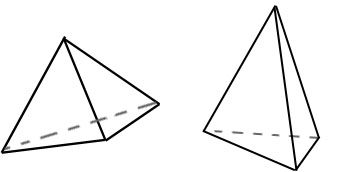
\includegraphics[width=0.35\textwidth]{ImgTetrahedrons.jpg}
  \end{center}
\end{figure}
Consider the tetrahedron that is bounded by the three coordinate planes in $\R^3$, and by the plane $z = 1 - x - \frac{y}{2}$.
\BEN
\item Sketch the tetrahedron in $\R^3$ and label the points that represent its four vertices. 
\item Set up, but do not evaluate, a double integral that represents the volume of the tetrahedron. Integrate with respect to $x$ first. 
\item Set up, but do not evaluate, a double integral that represents the volume of the tetrahedron. Integrate with respect to $y$ first. 
\EEN
Note that
\begin{itemize}
\item Examples 3.4 and 3.5 from \VCT \ are similar to this problem. 
\item We could also calculate the volume of the solid by using a \Emph{triple} integral. 
\item Although not required, the double integrals are straightforward to compute. You may want to check your answers by evaluating the integrals and seeing if you would get the same result in parts (b) and (c). 
\end{itemize}
% ~~~~~~~~~~~~~~~~~~~~~~~~~~~~~~~~~~~~~~~~~~~~~~~~~~~~~~~~~~~~~~~~~~~~~~~~~~~~~~~~~
\item  % DESCRIBE WHY A PARTICULAR DOUBLE INTEGRAL GIVES AREA
\Emph{Area of a General Region}
\BEN
\item Solve Question 11 from Section 3.2 of \VCT, which is
\begin{quotation}
\noindent
Explain why the double integral $\iint_R 1 dA$ gives the area of the region $R$. For simplicity, you can assume that $R$ is a region of the type shown in Figure 3.2.1(a).
\end{quotation}
\textit{Additional hint: Figure 3.2.5 is also helpful.}
\item Use the result from part (a) to compute the area of the region bounded by the curves $y = x^2$ and $x=y^2$.
\EEN

% ~~~~~~~~~~~~~~~~~~~~~~~~~~~~~~~~~~~~~~~~~~~~~~~~~~~~~~~~~~~~~~~~~~~~~~~~~~~~~~~~~
\item % UPPER AND LOWER BOUNDS ARE FUNCTIONS
Find the volume of the solid enclosed by $z = x^2 + y^2$, $y = x^2$ and $x=y^2$.
% ~~~~~~~~~~~~~~~~~~~~~~~~~~~~~~~~~~~~~~~~~~~~~~~~~~~~~~~~~~~~~~~~~~~~~~~~~~~~~~~~~
\item % CHANGING ORDER OF INTEGRATION
Consider the integral
\begin{align*}
  \iint\limits_R x\sin(y) dA
\end{align*}
 where $R$ is the region bounded by $y=0$, $y=x^2$, and $x=2$.
\BEN
\item Evaluate the double integral by first integrating with respect to $x$. 
\item Evaluate the double integral by first integrating with respect to $y$. 
\EEN
Note that your answers for both parts should be the same, and that you may need to use various techniques of integration to complete this problem, including integration by parts and a variable substitution. 
% ~~~~~~~~~~~~~~~~~~~~~~~~~~~~~~~~~~~~~~~~~~~~~~~~~~~~~~~~~~~~~~~~~~~~~~~~~~~~~~~~~
\item % CHANGING ORDER OF INTEGRATION, GENERAL F(X,Y)
\textbf{Changing the Order of Integration} \\
Consider the double integral
\begin{align*}
  \mathop{\int_{0}^{1+e} \! \int_0^{\ln(x-1)}} f(x,y) dydx .
\end{align*}
Sketch the region in $\R^2$ over which $f(x,y)$ is integrated, and change the order of integration.  
% ~~~~~~~~~~~~~~~~~~~~~~~~~~~~~~~~~~~~~~~~~~~~~~~~~~~~~~~~~~~~~~~~~~~~~~~~~~~~~~~~~
\item % BOUNDING AN INTEGRAL 
\textbf{Bounding A Double Integral} \\
Consider the double integral
\begin{align*}
  \iint\limits_D f(x,y) dA,
\end{align*}
where $D$ is the square $0\le x \le 1$, $0\le y \le 1$, and $f(x,y) = \sin(x+y)$. Show that 
\begin{align*}
  0 \le \iint\limits_D f(x,y) dA \le 1.
\end{align*}
% ~~~~~~~~~~~~~~~~~~~~~~~~~~~~~~~~~~~~~~~~~~~~~~~~~~~~~~~~~~~~~~~~~~~~~~~~~~~~~~~~~
\item % SYMMETRY
\textbf{Simplifying Double Integrals Using Symmetry} \\
Certain integrals can be simplified when the integrand is either even or odd. You may know that, for functions of one variable, that
\begin{align*}
  \text{if }f(x)\text{ is odd, then } & \int_{-a}^{a} f(x) dx = 0 . \\
  \text{if }f(x)\text{ is even, then } & \int_{-a}^{a} f(x) dx = 2 \int_0^a f(x) dx.
\end{align*}
There are similar results for integrals of two variables, but in order to introduce them, we first need to extend our concepts of even and odd functions to functions of two variables, and we need to describe regions that are symmetric about the $x$-axis and about the $y$-axis. 

If $R$ is a region that is \Emph{symmetric about the $y$-axis}, and $(x_0,y_0)$ is a point inside $R$, then the point $(-x_0,y_0)$ is also inside $R$. Similarily, if $S$ is a region that is \Emph{symmetric about the $x$-axis}, and $(x_1,y_1)$ is a point inside $S$, then the point $(x_1,-y_1)$ is also inside $S$. Above are examples of regions that have these symmetries.\\

\begin{figure}[h]
  \vspace{-1pt}
  \begin{center}
    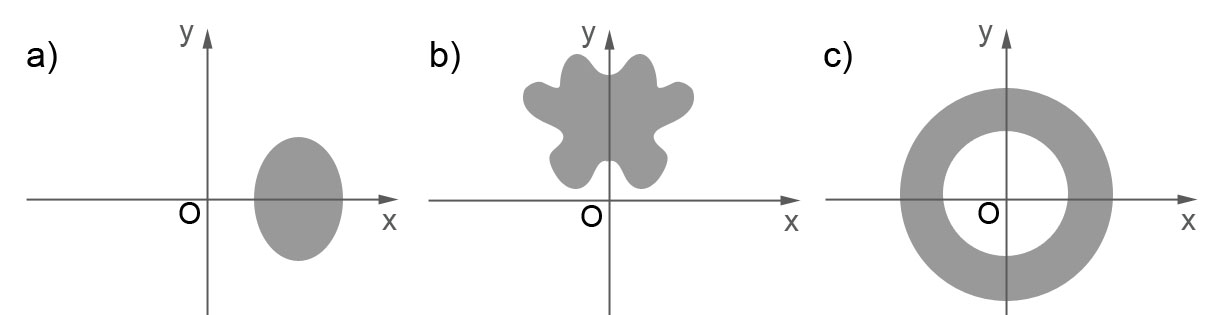
\includegraphics[width=0.95\textwidth]{ImgRegions.jpg}
  \end{center}
 \begin{quote} \caption{\small{a) the grey region is symmetric about the $x$-axis, b) the grey region is symmetric about the $y$-axis, and c) the grey region is symmetric about the $x$-axis and the $y$-axis.}}\end{quote}
\end{figure}

Moreover, if $g(x,y)$ is odd in $x$, then 
\begin{align*}
  g(-x,y) = - g(x,y).
\end{align*}
But if $g(x,y)$ were even in $x$, then 
\begin{align*}
  g(-x,y) =  g(x,y).
\end{align*}
Combining these concepts yields helpful results for computing double integrals. For example, if $R$ is symmetric about the $y$-axis, and if $g(x,y)$ is odd in $x$, then
\begin{align*}
  \iint\limits_R g(x,y) dxdy = 0.
\end{align*}
Similar results can be stated if $g$ were even in $x$ or in $y$, and if $R$ has symmetry about the $x$-axis. 
\BEN
\item Provide an example of a non-zero function of two variables, $h(x,y)$, that is odd in $x$. Verify that your function is odd in $x$.
\item Provide an example of a region, $D$, that is symmetric about the $y$-axis, but is not symmetric about the $x$-axis. 
\item Show that, for your $h(x,y)$ and region $D$, that 
\begin{align*}
  \iint\limits_D g(x,y) dxdy = 0.
\end{align*}
\EEN

% ~~~~~~~~~~~~~~~~~~~~~~~~~~~~~~~~~~~~~~~~~~~~~~~~~~~~~~~~~~~~~~~~~~~~~~~~~~~~~~~~~
\EEN % END OF SUBSECTION
